\begin{savequote}[8cm]
\textlatin{Neque porro quisquam est qui dolorem ipsum quia dolor sit amet, consectetur, adipisci velit...}

There is no one who loves pain itself, who seeks after it and wants to have it, simply because it is pain...
  \qauthor{--- Cicero's \textit{de Finibus Bonorum et Malorum}}
\end{savequote}

\chapter{\label{ch:3-t2k}The T2K Experiment} 

\minitoc
The T2K experiment is a long-baseline neutrino experiment, aiming to measure CP violation in the lepton sector through neutrino oscillation measurement.
This chapter will first describe the experimental setup and provide a brief overview of the software, which forms the ground for understanding and discussion of the subsequent analyses.


\section{Hardware}
As a long-baseline experiment, T2K is comprised of a near detector, ND280, and a far detector, Super-Kamiokande (SK).
To measure neutrino oscillation, both detectors need to be able to distinguish between $\numu$ and $\nue$.  
Of course, no detectors can detect neutrinos directly.
In practice, both detectors should possess the capability to distinguish well the different products from neutrino interaction with the active material of the detectors.
The most common products of neutrino-nucleus interactions are the corresponding leptons, i.e. electron and muon, and several hadrons, including protons, nucleons and light mesons like pions.

The far detector, SK, is a huge water Cherenkov detector.
It detects the presence of particles by capturing the Cherenkov light emitted due to their superluminal motion in water.
Hadrons produced in neutrino interactions are not energetic enough to emit Cherenkov radiation, while the leptons typically are able to travel faster than light.
Thus, SK mainly measure electrons and muons.
The Cherenkov radiation from these leptons typically forms a ring-like pattern perpendicular to the particle motion.
Due to the lighter mass of the electron, its propagation direction is more likely to change due to scattering along its motion than muon.
Hence, the Cherenkov ring from an electron is more diffuse than that from a muon, as shown in Fig.~\ref{fig:sk-e-mu}.

    \begin{figure}
          \centering
          \begin{subfigure}[b]{\dbfigwid\textwidth}
               \centering
               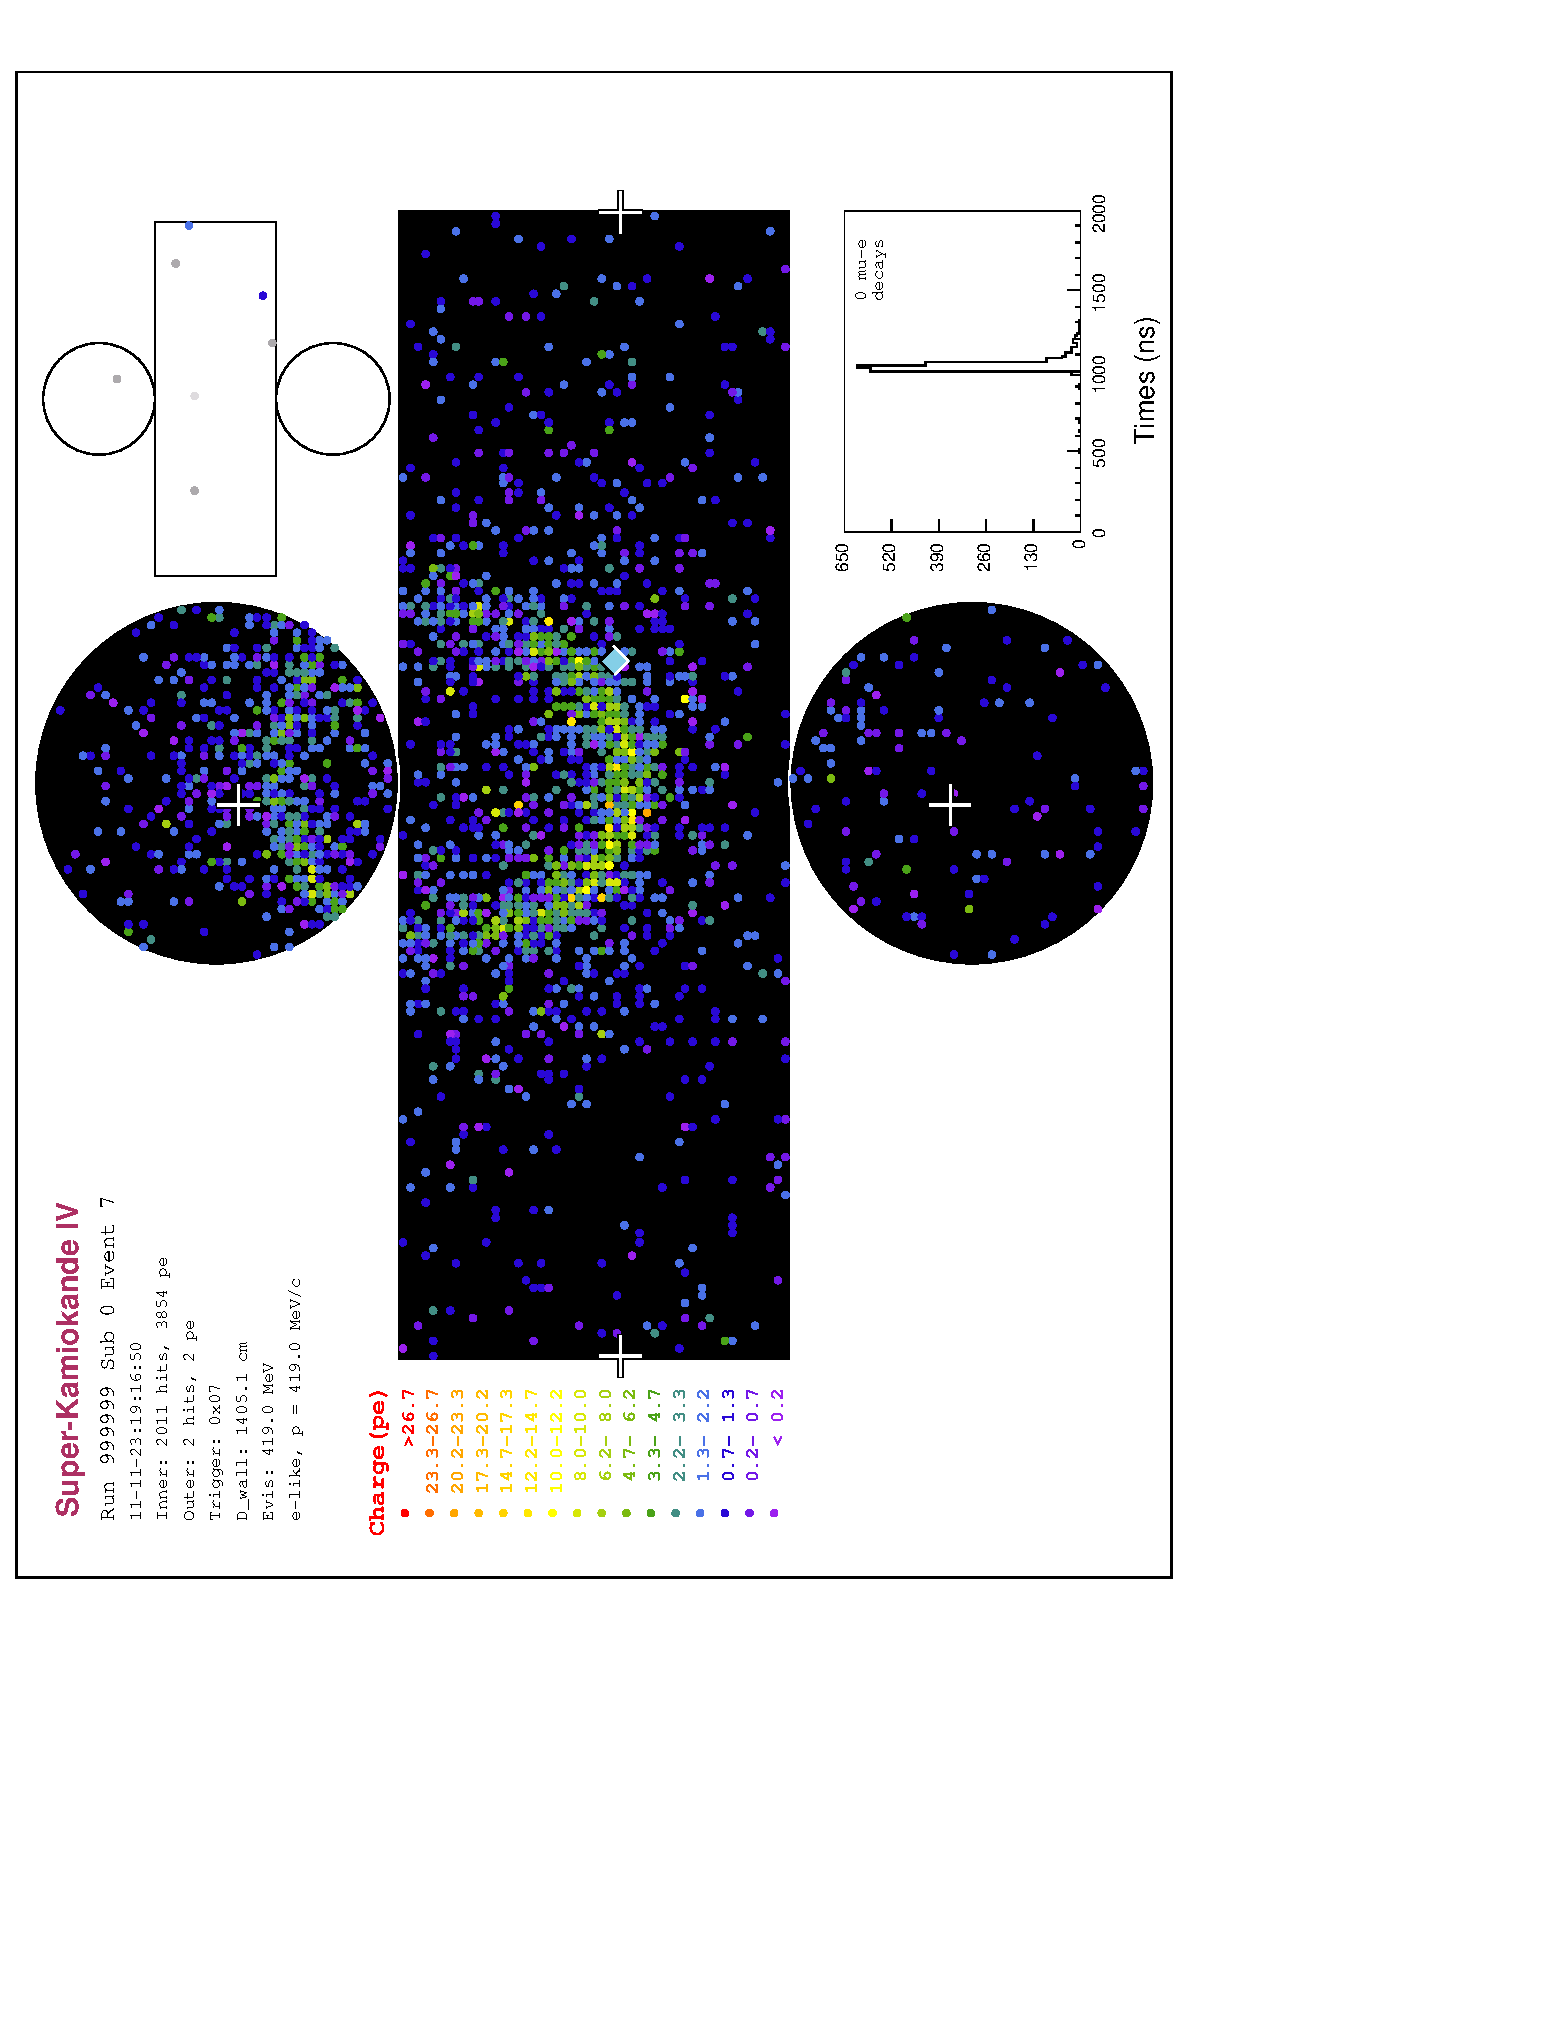
\includegraphics[width=\dbfigwid\textwidth]{figures/t2k/sk-nue.eps}
               \caption{nue}
               \label{subfig:sk-nue}
          \end{subfigure}
          \begin{subfigure}[b]{\dbfigwid\textwidth}
               \centering
               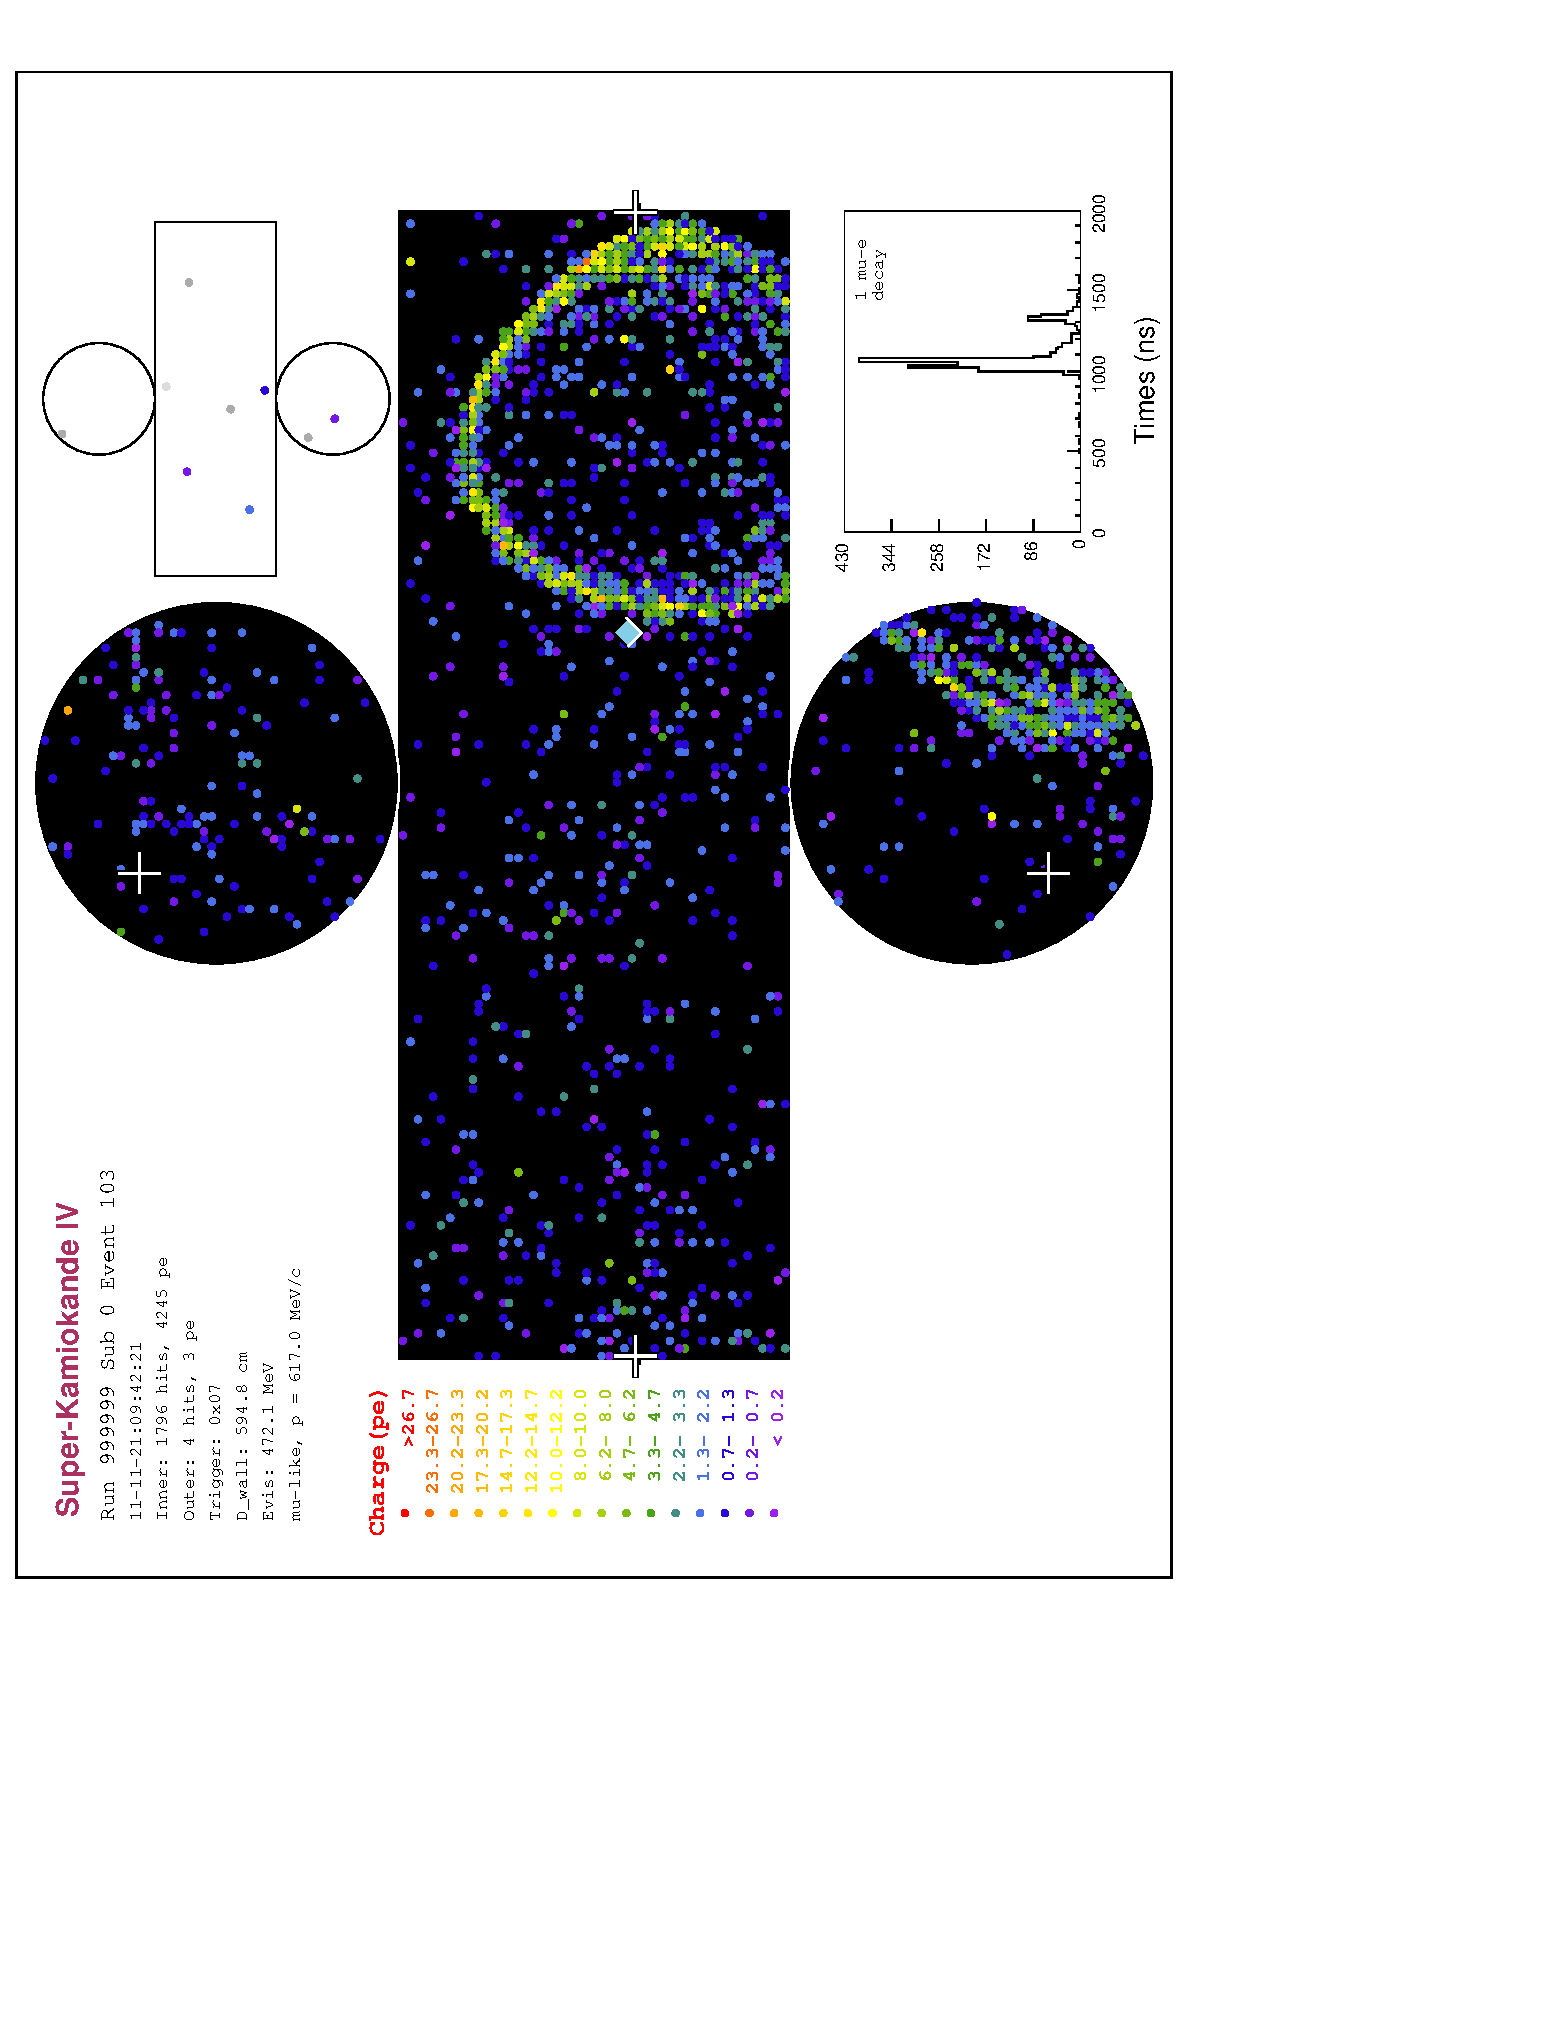
\includegraphics[width=\dbfigwid\textwidth]{figures/t2k/sk-numu.eps}
               \caption{numu}
               \label{subfig:sk-numu}
          \end{subfigure}
          \caption{SK event displays.}
          \label{fig:sk-e-mu}
    \end{figure}


More specifically, $\dcp$ can be measured in long-baseline neutrino experiments, for example, the Tokai-to-Kamioka (T2K) experiment\cite{T2KEXP}. 
T2K is a long-baseline neutrino experiment located in Japan. 
The neutrino source is generated in J-PARC in Tokai. 
A near detector, ND280, is placed at $280\mathrm{m}$ from the generation point, and a far detector, the Super Kamiokande (SK), is situated 296km away. As neutrinos interact extremely weakly, direct measurement is not yet possible. These detectors measure the neutrino energy spectra from the product particles from the interaction between neutrinos and hydrocarbons in ND280 and water molecules in SK. The difference between neutrino oscillation and anti-neutrino oscillation can be measured by comparing the neutrino energy spectra observed at the far and near detectors in the neutrino mode and the anti-neutrino mode. In 2020, the Tokai-to-Kamioka (T2K) experiment\cite{T2KEXP} has made the first measurement of $\dcp$\cite{T2Knature}, which ruled out CP conservation at the $95\%$ confidence level. It is an impressive first step, but it is still limited both by statistical and systematic uncertainties. 

 
\subsection{\label{sec:ndup} ND280 Upgrade}
   In the upgrade, the $\piz$ detector is replaced by a suite of sophisticated new sub-detectors, namely the Time-of-flight detector (TOF), two high angle TPCs and the Super Fine Grained Detector (SFGD). 
   The TOF consists of 6 planes of scintillation bars, providing excellent sub-nano second timing resolution. 
   It can effectively veto trespassing particles, thus improving the sample purity.
   The high angle TPCs (HAT) have a new field cage design and new Micromegas, leading to a larger tracking volume and better resolution than the existing vertical TPCs in ND280. 
   The SFGD is the new active target, consisting of about 2 million scintillation cubes, each with a size of $1~\textrm{cm}^3$. 
   The granularity of SFGD improves the high-angle acceptance significantly and thus leads to better phase space matching between the ND and the FD. 
   Moreover, the tracking capabilities are also enhanced by the more precise measurement of energy deposited along the particle track. 
   Hence, detection thresholds are lowered and resolution improved, opening up avenues for novel reconstruction techniques, such as trackless pion reconstruction, and creative construction of variables, like COM variables. 
   The upgrade has finished in April 2024 and the upgraded detector has started taking data in June 2024. An example event display is shown in Fig.~\ref{fig:ndup-evedis}. 

    \begin{figure}[!htb]
        \centering
        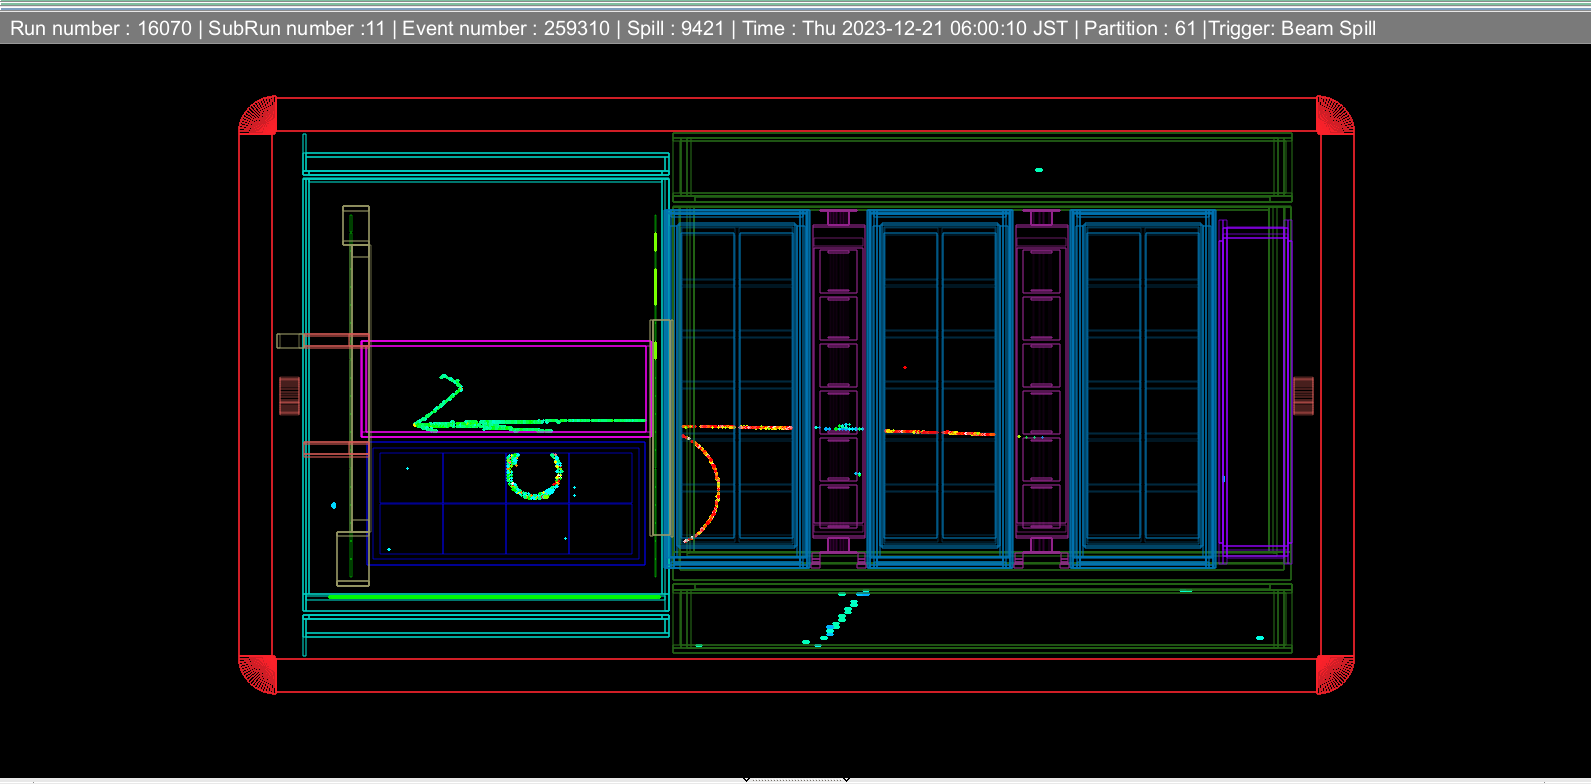
\includegraphics[width=0.5\linewidth]{fig/upgradeEvtDis.png}
        \caption{Event display of a possible $\pi^+$ event.}
        \label{fig:ndup-evedis}
    \end{figure}

\section{Software}
  \label{sec:t2k-sw}
  As a considerable portion of this thesis consists of improvement made on reconstruction performance, it is also apt to provide an overarching introduction to the reconstruction framework implemented for the T2K ND upgrade to aid understanding of the content follows.

  Each scintillation fibre in the SFGD constitutes a electronic signal channel.
  Hence, scintillation photons produced as a particle travels through the cubes are collected by the three planes of electronic boards on the three sides of SFGD.
  These electronic signal will be converted to digital singals after calibration.
  The three 2-dimensional planes of signals are then combined into one collectiion of 3-dimensional "Hits", each of which corresponds to a cube, with a 3-dimensional coordinate and a number of charges deposited. 
  These "Hits" are then passed through a combination of grouping and track-fitting algorithms, which collects the Hits into physically identifiable objects, namely clusters and tracks. 
  Clusters are isolated objects, which are not long enough to form a track, usually with less than 3 Hits.
  Tracks, on the other hand, contain many more Hits. 
  However, as the optical insulation coating on the cube is not perfect, there bounds to be leakage of photons to the neighbouring cubes that the particle has not actually passed by.
  Hence, the reconstruction algorithm also combines neighbouring Hits into Nodes, which reflect the particle trajectory more closely.
  Besides, the energy deposited at each Node is also estimated from the charges deposited at the constituent Hits and is further smoothed due to physical considerations that the energy deposited along a particle trajectgory is expected to be continuous.
  The smoothed energy along with other accessible information is passed through a Boosted Decision Tree (BDT) algorithm, trained on Particle Gun (PGUN) simulations, for particle identification and momentum reconstruction.
